\documentclass[aspectratio=169]{beamer}
\usepackage{booktabs}
\usepackage{xcolor}
\usepackage{changepage}
\usepackage[export]{adjustbox}
\usepackage{booktabs}
\usepackage{graphbox}
\usepackage[absolute,overlay]{textpos}
\usepackage{minted}
\usepackage{mdframed}

\usetheme[numbering=fraction,progressbar=frametitle]{metropolis}


% Backup
\newcommand{\backupbegin}{
   \newcounter{finalframe}
   \setcounter{finalframe}{\value{framenumber}}
}
\newcommand{\backupend}{
   \setcounter{framenumber}{\value{finalframe}}
}


% Colors
\definecolor{myBlue}{RGB}{21, 56, 110}
\definecolor{myRed}{RGB}{174,0,34}
\definecolor{myRedBg}{RGB}{251, 217, 224}
\definecolor{greySAS}{RGB}{167,166,166}
\definecolor{greyCU}{RGB}{44,46,53}

\setbeamercolor{title}{fg=myBlue}
\setbeamercolor{background canvas}{bg=white}
\setbeamercolor{normal text}{fg=black}
\setbeamercolor{frametitle}{fg=myBlue, bg=white}
\setbeamercolor{section title}{fg=myBlue}
\setbeamercolor{title separator}{fg=myRed,bg=myRedBg}
\setbeamercolor{progress bar}{fg=myRed,bg=myRedBg}
\setbeamercolor{structure}{fg=myRed}


% Frame around codeblocks
\surroundwithmdframed{minted}


% Thicker progress bar
\makeatletter
\setlength{\metropolis@titleseparator@linewidth}{1pt}
\setlength{\metropolis@progressonsectionpage@linewidth}{1pt}
\setlength{\metropolis@progressinheadfoot@linewidth}{1pt}
\makeatother


% Commands
\newcommand{\bluetext}[1]{%
  \textcolor{myBlue}{#1}
}
\newcommand{\redtext}[1]{%
  \textcolor{myRed}{#1}
}
\newcommand{\vtype}[1]{%
  \textcolor{myBlue}{\texttt{#1}}
}


% Title
\title{PandoraPFA for FCC-ee LAr Calorimeter}
\author{Juraj~Smie\v{s}ko\inst{1,2}}
\institute{\inst{1} Charles University, Czechia \\
           \inst{1} CERN}
\date{\footnotesize
      Workshop on GranuLAr noble liquid detectors \\
      08 Apr 2022}

%
% -----------------------------------------------------------------------------
%
\begin{document}


{%
  \setbeamercolor{background canvas}{bg=greyCU}
  \begin{frame}[noframenumbering]
    \centering
    \vspace{1cm}
    
\includegraphics[width=.25\textwidth]{figures/CU_red_white_logo.pdf}
    \thispagestyle{empty}
  \end{frame}
}

\begin{frame}
  \titlepage{}
  \thispagestyle{empty}
\end{frame}

\begin{frame}
  \frametitle{\bf Particle Flow}

  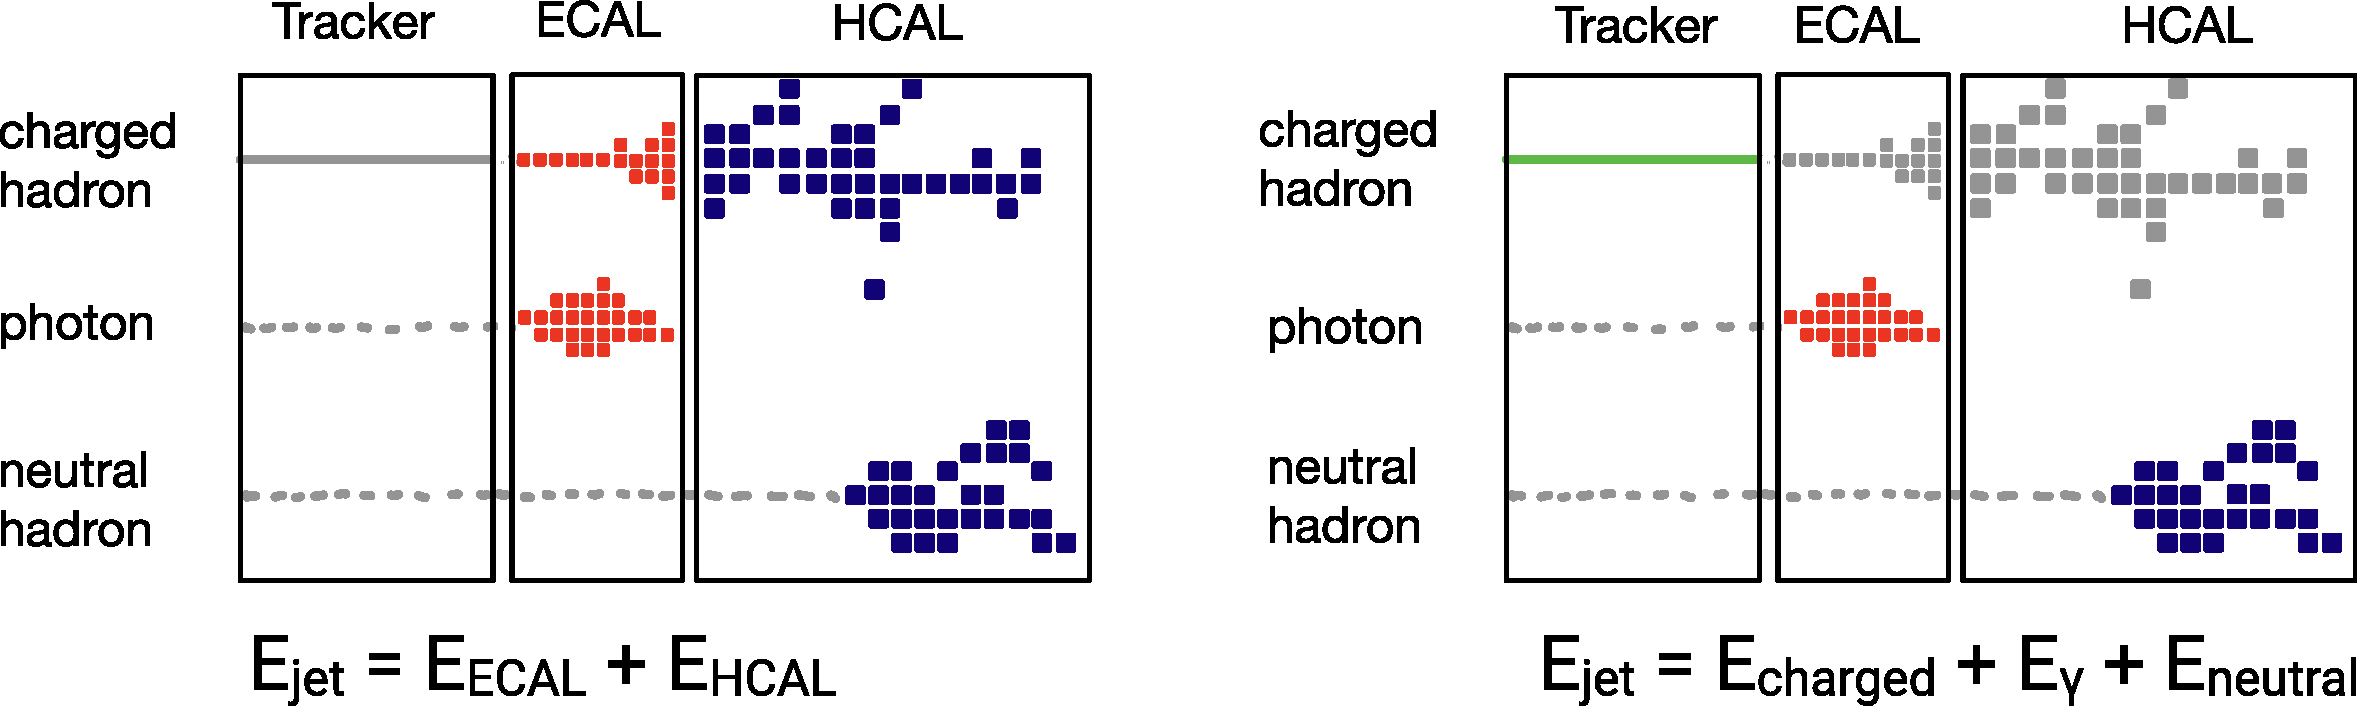
\includegraphics[width=\linewidth]{figures/particle_flow_diagram.pdf}
  \vspace{-1.5ex}
  \hspace{6.7em} 30\% + 70\% \hspace{14.5em} 60\% + 30\% + 10\%

  \begin{columns}[c]
    \column{.5\textwidth}
    \begin{itemize}
      \item Reconstruct every particle in the event with the best possible
            precision
      \item Combine the measurements in subdetectors in an optimal way
    \end{itemize}

    \column{.5\textwidth}
    \begin{itemize}
      \item Charged particles dominated by tracker
      \item Calorimetry mostly for neutral particles
      \item \bluetext{\bf Enemy: Confusion}
    \end{itemize}
  \end{columns}

  \begin{textblock*}{\paperwidth}(4pt, 0.15\textheight)
    \tiny
    \href{https://indico.cern.ch/event/932973/}
         {source}
  \end{textblock*}
\end{frame}


\begin{frame}[fragile]
  \frametitle{PandoraPFA I.}

  \begin{itemize}
    \item Framework which employs multitude of pattern recognition algorithms
      to \bluetext{\bf form/manipulate clusters} and \bluetext{\bf create PFOs}
      (particle flow objects)
    \item To facilitate different algorithms there are several layers
    \item The algorithms can be selected in a steering xml
  \end{itemize}


  \begin{columns}[c]
    \column{.55\textwidth}

    \begin{center}
      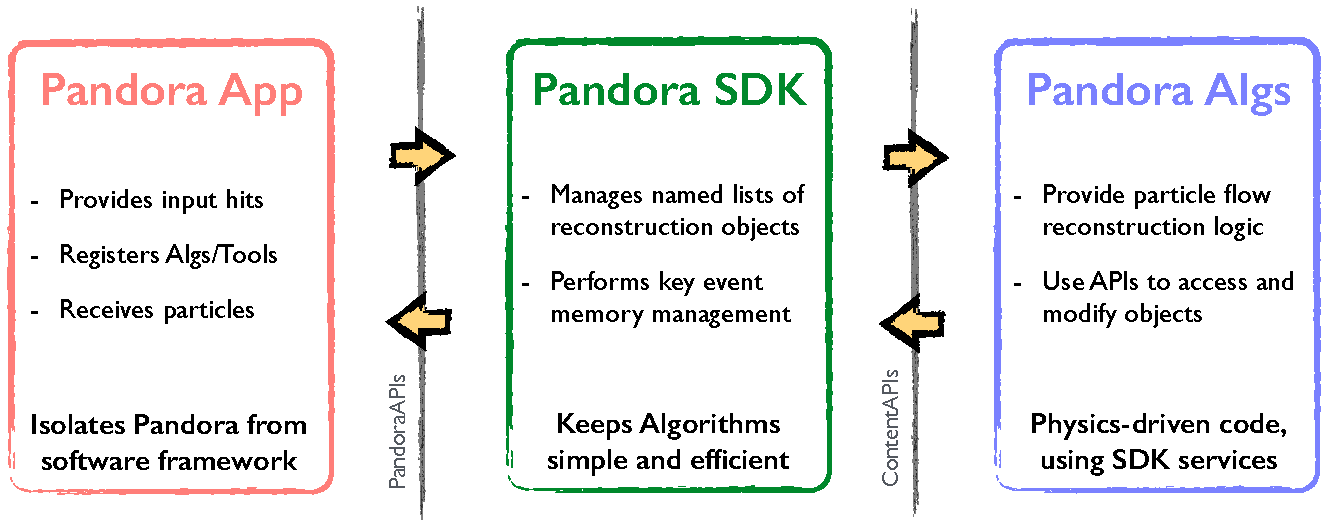
\includegraphics[width=\textwidth]{figures/pandora_apis.pdf}
    \end{center}

    \column{.45\textwidth}

    \fontsize{5}{8} \selectfont
    \begin{minted}{xml}
<algorithm type = "ConeClustering" instance = "Reclustering1">
    <TanConeAngleFine>0.24</TanConeAngleFine>
    <TanConeAngleCoarse>0.4</TanConeAngleCoarse>
    <AdditionalPadWidthsFine>2</AdditionalPadWidthsFine>
    <AdditionalPadWidthsCoarse>2</AdditionalPadWidthsCoarse>
    <SameLayerPadWidthsFine>2.24</SameLayerPadWidthsFine>
    <SameLayerPadWidthsCoarse>1.44</SameLayerPadWidthsCoarse>
    <MaxTrackSeedSeparation>100</MaxTrackSeedSeparation>
    <MaxLayersToTrackSeed>0</MaxLayersToTrackSeed>
    <MaxLayersToTrackLikeHit>0</MaxLayersToTrackLikeHit>
    <TrackPathWidth>0</TrackPathWidth>
</algorithm>
    \end{minted}
  \end{columns}


  \begin{textblock*}{\paperwidth}(4pt, 1.1\textheight)
    \tiny
    \href{https://github.com/PandoraPFA/Documentation/blob/master/Pandora_Example.pdf}
         {source}
  \end{textblock*}
\end{frame}


\begin{frame}
  \frametitle{PandoraPFA II.}

  \begin{center}
    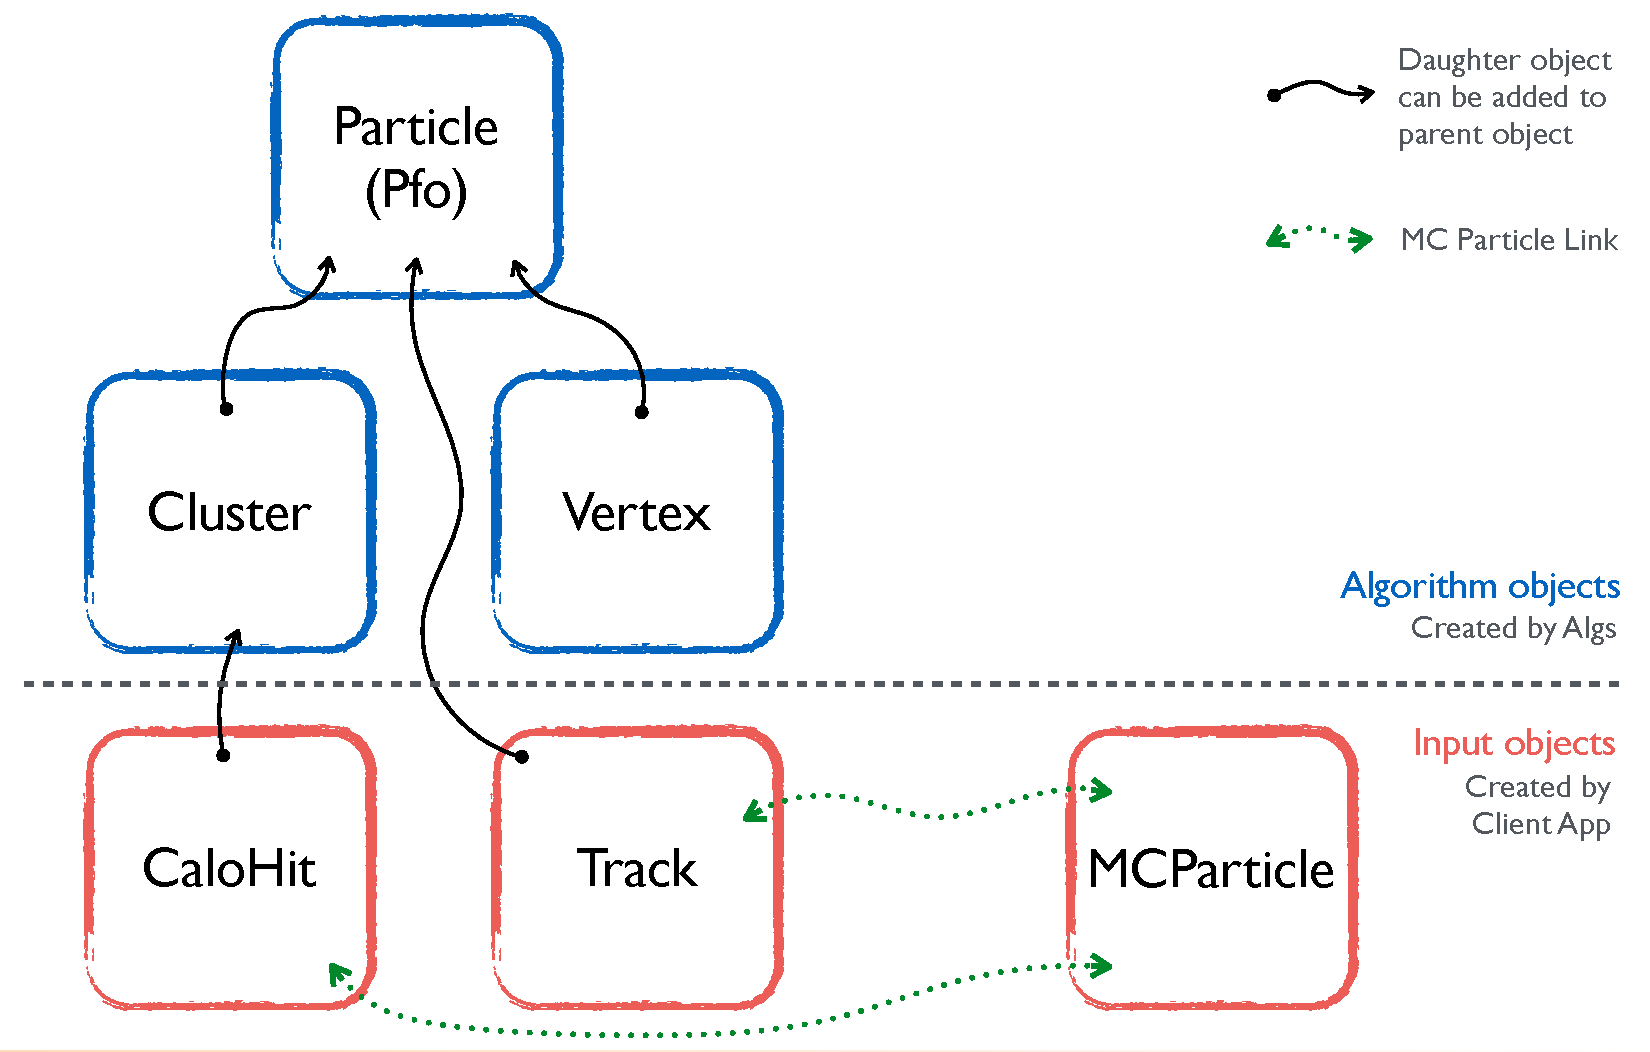
\includegraphics[width=.8\textwidth]{figures/pandora_edm.pdf}
  \end{center}

  \begin{textblock*}{\paperwidth}(4pt, 0.15\textheight)
    \tiny
    \href{https://github.com/PandoraPFA/Documentation/blob/master/Pandora_Example.pdf}
         {source}
  \end{textblock*}
\end{frame}


\begin{frame}
  \frametitle{Wrappers}

  \begin{columns}[c]
    \column{.5\textwidth}

    \bluetext{\bf DDMarlinPandora}

    \begin{itemize}
      \item Developed for ILC
      \item Pandora application wrapped inside Marlin processor
      \item Conversion between LCIO and Pandora datamodel
            \begin{itemize}
              \item CaloHits
              \item Tracks
              \item MCParticles
              \item Geometry
            \end{itemize}
      \item Provides xml settings file
    \end{itemize}

    \column{.5\textwidth}

    \bluetext{\bf k4MarlinWrapper}
    \begin{itemize}
      \item Wraps Marlin processor inside Gaudi algorithm
      \item Converts from EDM4hep datamodel into LCIO datamodel
      \item Marlin processor is steered by python script instead of xml file
    \end{itemize}
  \end{columns}
\end{frame}


\begin{frame}[fragile]
  \frametitle{The Plan for Running Pandora}

  \begin{center}
    \texttt{\bluetext{k4MarlinWrapper}}
    $\leftrightarrow$ \texttt{\bluetext{DDMarlinPandora}}
    $\leftrightarrow$ \bluetext{\bf Pandora}
  \end{center}

  \begin{columns}[c]
    \column{.55\textwidth}

    \begin{itemize}
      \item Considered to be \bluetext{\bf quickest} way to have Pandora running
      \item \redtext{\bf Disadvantage:} two datamodel conversions
      \item Over time, development of the native Key4hep wrapper
      \item \bluetext{\bf First step:} Get just Pandora clustering algorithm run
    \end{itemize}

    \column{.45\textwidth}

    \tiny
    \begin{minted}{python}
from Configurables import MarlinProcessorWrapper

pandora = MarlinProcessorWrapper('DDMarlinPandora')
pandora.OutputLevel = DEBUG
pandora.ProcessorType = 'DDPandoraPFANewProcessor'
pandora.Parameters = {
    'Verbosity': ['WARNING'],
    'PandoraSettingsXmlFile': ['/some/path'],
    'CreateGaps': [False],
    'ECalCaloHitCollections': ['ECalBarrelCells']
}
ApplicationMgr().TopAlg += [pandora]
\end{minted}
  \end{columns}
\end{frame}


\begin{frame}
  \frametitle{EDM Conversions: CaloHits I}

  \resizebox{\textwidth}{!} {
    \begin{tabular}{lll}
      \bluetext{\bf Pandora} & \bluetext{\bf LCIO | CalorimeterHitImpl}
                             & \bluetext{\bf EDM4hep | ReconstructedParticle} \\
      \vtype{CartesianVector} m\_positionVector
        & \vtype{float} \_position[3]
        & \vtype{edm4hep::Vector3f} position \\
      \vtype{float} m\_x0 & \\
      \vtype{const CartesianVector} m\_expectedDirection & \\
      \vtype{const CartesianVector} m\_cellNormalVector; & \\
      \vtype{const CellGeometry} m\_cellGeometry \\
      \vtype{const float} m\_cellSize0 & \vtype{int} \_cellID0
                                       & \vtype{uint64\_t} cellID \\
      \vtype{const float} m\_cellSize1 & \vtype{int} \_cellID1 \\
      \vtype{const float} m\_cellThickness \\
      \vtype{const float} m\_nCellRadiationLengths \\
      \vtype{const float} m\_nCellInteractionLengths; \\
      \vtype{const float} m\_time & \vtype{float} \_time
                                  & vtype{float} time \\
      \vtype{const float} m\_inputEnergy & \vtype{float} \_energy
                                         & \vtype{float} energy \\
      \vtype{const float} m\_mipEquivalentEnergy \\
      \vtype{const float} m\_electromagneticEnergy \\
      \vtype{const float} m\_hadronicEnergy \\
      \vtype{const bool} m\_isDigital \\
    \end{tabular}
  }
\end{frame}


\begin{frame}
  \frametitle{EDM Conversions: CaloHits II}

  \resizebox{\textwidth}{!} {
    \begin{tabular}{lll}
      \bluetext{\bf Pandora} & \bluetext{\bf LCIO | CalorimeterHitImpl}
                             & \bluetext{\bf EDM4hep | ReconstructedParticle} \\
      \vtype{const HitType} m\_hitType & \vtype{int} \_type
                                       & \vtype{int32\_t} type \\
      \vtype{const HitRegion} m\_hitRegion \\
      \vtype{const unsigned int} m\_layer \\
      \vtype{InputUInt m\_pseudoLayer} \\
      \vtype{const bool} m\_isInOuterSamplingLayer \\
      \vtype{float} m\_cellLengthScale \\
      \vtype{bool} m\_isPossibleMip \\
      \vtype{bool} m\_isIsolated \\
      \vtype{bool} m\_isAvailable \\
      \vtype{float} m\_weight \\
      \vtype{MCParticleWeightMap}  m\_mcParticleWeightMap \\
      \vtype{const void} *m\_pParentAddress \\
    \end{tabular}
  }
\end{frame}


\begin{frame}
  \frametitle{EDM Conversions: PFOs $\leftrightarrow$ EDM4hep}

  \resizebox{\textwidth}{!} {
    \begin{tabular}{lll}
      \bluetext{\bf EDM4hep | ReconstructedParticle}
        & \bluetext{\bf LCIO | ReconstructedParticleImpl}
        & \bluetext{\bf Pandora | ParticleFlowObject} \\
      \vtype{int32\_t} type & \vtype{int} \_type & \vtype{int} m\_particleId \\
      \vtype{float} energy & \vtype{double} \_energy & \vtype{float} m\_energy \\
      \vtype{edm4hep::Vector3f} momentum & \vtype{double} \_momentum[3] & \vtype{CartesianVector} m\_momentum \\
      \vtype{edm4hep::Vector3f} referencePoint & \vtype{float} \_reference[3] & \\
      \vtype{float} charge & \vtype{float} \_charge & \vtype{int} m\_charge \\
      \vtype{float} mass & \vtype{double} \_mass & \vtype{float} m\_mass \\
      \vtype{float} goodnessOfPID & \vtype{float} \_goodnessOfPID & \\
      \vtype{std::array<float,10>} covMatrix & \vtype{EVENT::FloatVec} \_cov & \\
      %OneToOneRelations: & & \\
      \vtype{edm4hep::Vertex} startVertex & \vtype{EVENT::Vertex*} \_sv & \vtype{VertexList} m\_vertexList \\
      \vtype{edm4hep::ParticleID} particleIDUsed & \vtype{EVENT::ParticleID*} \_pidUsed & \\
      %OneToManyRelations: & & \\
      \vtype{edm4hep::Cluster} clusters & \vtype{EVENT::ClusterVec} \_clusters & \vtype{ClusterList} m\_clusterList \\
      \vtype{edm4hep::Track} tracks & \vtype{EVENT::TrackVec} \_tracks & \vtype{TrackList} m\_trackList \\
      \vtype{edm4hep::ReconstructedParticle} particles &
      \vtype{EVENT::ReconstructedParticleVec} \_particles & \\
      \vtype{edm4hep::ParticleID} particleIDs & \vtype{EVENT::ParticleIDVec} \_pid & \\
      & & \vtype{PfoList} m\_parentPfoList \\
      & & \vtype{PfoList} m\_daughterPfoList \\
      & & \vtype{PropertiesMap} m\_propertiesMap \\
%     MutableExtraCode:
%       declaration: "
%       bool isCompound()
% 
    \end{tabular}
  }
\end{frame}


\begin{frame}
  \frametitle{What is Missing?}

  \scriptsize
  PandoraPFA/\texttt{DDMarlinPandora} requires following components:

  \vspace{-1ex}

  \begin{itemize}\scriptsize
    \item \bluetext{Geometry description in DD4HEP format}
          \begin{itemize}\scriptsize
            \item IDEA-LAr already described in it, needs code to build
                  instance in memory
          \end{itemize}
   \item \bluetext{Calorimeter hits}
          \begin{itemize}\scriptsize
            \item Conversions provided by
                  \texttt{DDMarlinPandora}/\texttt{k4MarlinWrapper}
          \end{itemize}
          % \begin{itemize}
          %   \item Conversion from LCIO datamodel to Pandora datamodel provided
          %         by \texttt{DDMarlinPandora} wrapper
          %   \item Conversion from EDM4hep datamodel provided by
          %         \texttt{k4MarlinWrapper}
          % \end{itemize}
    \item \redtext{Tracks alongside with vertexes}
          \begin{itemize}\scriptsize
            \item Requires custom code, base class provided
          \end{itemize}
    \item \bluetext{MCParticles}
          \begin{itemize}\scriptsize
            \item Conversions provided by
                  \texttt{DDMarlinPandora}/\texttt{k4MarlinWrapper}
          \end{itemize}
  \end{itemize}

  Also required are:

  \vspace{-1ex}

  \begin{itemize}\scriptsize
      \item Conversion of PFOs from Pandora datamodel
          \begin{itemize}\setlength{\itemsep}{.5ex}\scriptsize
            \item Conversions provided by
                  \texttt{DDMarlinPandora}/\texttt{k4MarlinWrapper}
          \end{itemize}
      \item Calibration of the calorimeter clusters
      \item Review of CLIC and ILD specific code
      \item Optimization of the algorithms / Setting correct parameters
  \end{itemize}
\end{frame}


\begin{frame}
  \frametitle{Conclusions}

  \begin{columns}[c]
    \column{.5\textwidth}

    \begin{itemize}
      \item Basic blocks are in place
      \item Let's start with just clustering to verify running of the whole chain
      \item ``Settings{}'' are the real challenge
            \begin{itemize}
              \item Detector parameters
              \item Calibrations
            \end{itemize}
    \end{itemize}

    \column{.5\textwidth}

    \begin{center}
      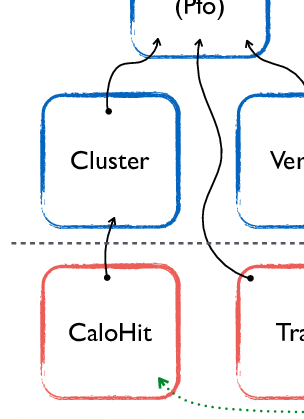
\includegraphics[width=.8\textwidth]{figures/pandora_edm_cut.png}
    \end{center}
  \end{columns}
\end{frame}



%
% -----------------------------------------------------------------------------
%
% \appendix
% \backupbegin{}
%
% \begin{frame}[c]
%   \begin{center}
%     \redtext{\Huge Backup}
%   \end{center}
% \end{frame}
%
%
%\backupend{}

\end{document}
